% !TeX root = main.tex
\section{Introdução}

Esse relatório corresponde a documentação sobre as conversas realizadas com uma LLM (Language Model) para discutir o escopo do projeto proposto para a disciplina de Inteligência Artificial. O objetivo principal foi avaliar uma base de dados de interesse e explorar possibilidades de algoritmos e técnicas de IA para a avaliação de aspectos específicos. Nesse sentido, com base em conhecimento prévio de um dos integrantes do grupo, explorou-se uma base de dados publicada na revista \textit{Nature Medicine} em 2021 sob o título \textit{Real-time alerting system for COVID-19 and other stress events using werable data} \cite{nature}. Sendo assim, a LLM foi questionada sobre o escopo do projeto, quais técnicas poderiam ser utilizadas, exploração do problema e das bases de dados envolvidas, entre outros aspectos relevantes relacionados. Segue abaixo a documentação da conversa realizada.

Destaca-se que a LLM utilizada para a exploração do problema foi o Gemini, na sua versão Pro, considerando a versão gratuita fornecida pela Google para estudantes.
\section{Histórico de conversa}
\begin{description}
    \item[Aluno:] Minha equipe possui o seguinte trabalho a ser desenvolvido na disciplina de inteligência artificial no contexto da engenharia de computação.

    Considere como contexto, o programa da disciplina:
    História da IA. Caracterização dos problemas de IA e aplicações (por exemplo, em processamento de linguagem natural, mineração de dados e robótica). Introdução à programação lógica e seu uso em IA. Métodos de busca para resolução de problemas: busca cega e informada, busca com adversários. Formalismos de representação de conhecimento e inferência: lógica, redes semânticas, frames, scripts e regras de produção. Sistemas baseados em conhecimento. Noções gerais de aprendizado de máquina. Introdução a algumas técnicas relevantes de aprendizado, como árvores de decisão, naive-bayes, redes neurais, algoritmos genéticos e k-means. Ética e impactos da IA.

    O projeto em questão será apresentado em uma feira científica voltada à alunos (feira de extensões ICMC). Considerando esse contexto, enviarei no próximo prompt a orientação do trabalho.

    \item[Gemini:] Contexto perfeitamente assimilado!

    A ementa da disciplina cobre uma base muito sólida, passando pelos fundamentos clássicos da IA (como métodos de busca, representação de conhecimento e sistemas baseados em regras) até os tópicos mais aplicados de aprendizado de máquina.

    Apresentar um projeto com essa profundidade técnica em uma feira de extensões do ICMC é uma excelente oportunidade. O grande desafio — e a parte mais legal — será traduzir a complexidade da Engenharia de Computação em algo que seja visualmente atrativo, interativo e fácil de entender para o público de estudantes, sem perder o rigor acadêmico nos bastidores.

    Estou a postos. Pode mandar as orientações do trabalho no próximo prompt para começarmos a estruturar as ideias!

    \item[Aluno:] Considere o enunciado do trabalho:
    ESPECIFICAÇÕES E DIRETRIZES

    Seleção de problema de IA generativa
    Busca fonte de dados (devemos buscar uma fonte aberta e ética de dados)
    Definição de paradigma
    Utilização extensa de IA para sugestão e refinamento do problema (professora solicitou que mostrássemos a nossa interação com a IA generativa).

    A especificação do trabalho consiste, de forma resumida, em encontrar um problema, buscar um conjunto de dados pertinente e resolvê-lo utilizando técnicas de aprendizado de máquina.
    Para realizar o trabalho, você deve seguir o pipeline de descoberta de conhecimento (ou a metodologia CRISP-DM), que engloba as seguintes etapas e regras:
    Identificação do Problema e Negócio: O ponto de partida é escolher um conjunto de dados e compreender profundamente o domínio e o contexto de negócio daquele problema.
    Pré-processamento e Extração de Padrões: Após preparar os dados (retirando vieses e inconsistências), você deverá aplicar algoritmos de aprendizado de máquina disponíveis (como KNN, algoritmos de regras de associação, agrupamento, etc.) para extrair padrões.
    A professora estabeleceu diretrizes claras sobre o uso de IAs generativas (como ChatGPT, Gemini, Claude, etc.) durante o desenvolvimento:
    Uso obrigatório para exploração: Você deve usar a IA na primeira etapa para explorar o problema, entender o contexto do negócio, questionar as respostas e expandir seu próprio conhecimento.
    Proibição na codificação central: Você não deve pedir para a IA escrever ou executar o algoritmo de mineração/aprendizado de máquina no seu lugar.
    Documentação rigorosa: Todo o uso feito de ferramentas de IA generativa deverá ser anexado e documentado no trabalho final. Será necessário detalhar quais ferramentas foram usadas, as datas, os prompts exatos que você criou e quem foi o responsável por validar as respostas geradas pela IA.

    Considere esse documento como pretexto para os próximos prompts, nos quais irei explorar tópicos possíveis e principalmente aprofundar o tópico de interesse.

    \item[Gemini:] Entendido! As regras do jogo estão muito claras e bem estruturadas. O foco aqui é seguir a metodologia CRISP-DM, garantir que a base de dados seja ética e aberta, e usar a IA como uma "parceira de brainstorming" estruturada. Ao mesmo tempo, a implementação central dos algoritmos de aprendizado de máquina (como KNN, regras de associação ou clustering) deve ser feita pela equipe, garantindo o rigor técnico da disciplina.

    Como o projeto será exposto em uma feira para alunos, temos a ótima oportunidade de escolher um problema que conecte a teoria de mineração de dados com aplicações visuais e interessantes para o público. Podemos explorar, por exemplo, o reconhecimento de padrões em interação humano-computador, a análise de dados de telemetria e navegação em robótica (talvez minerando dados para otimizar fluxos em árvores de comportamento), ou seguir por um caminho completamente diferente que gere bastante engajamento visual na feira.

    Estou pronto para atuar nessa etapa de Identificação do Problema e Negócio, aprofundando o contexto e questionando os caminhos, de forma que você tenha um material rico e detalhado para compor a sua documentação obrigatória de uso de IA.

    Para começarmos o nosso funil de ideias: você já tem algum domínio ou conjunto de dados específico em mente que gostaria de explorar primeiro, ou prefere que eu levante algumas opções de problemas e bases de dados abertas para analisarmos juntos?

    \item[Gemini:] Excelente escolha! A equipe tocou em um problema extremamente válido, com alto potencial prático e acadêmico.

    A detecção de doenças virais, como a Covid-19, através de dispositivos vestíveis (wearables) é um campo de pesquisa real e validado por instituições de ponta. Estudos como o \textit{CovIdentify} da Duke University e pesquisas da Stanford Medicine já demonstraram que a Frequência Cardíaca de Repouso (FCR) sofre uma elevação significativa dias antes dos primeiros sintomas aparecerem, devido ao estresse fisiológico causado pela inflamação.

    Abaixo, faço uma avaliação técnica da viabilidade da ideia, já estruturada na ótica da metodologia CRISP-DM para ajudar na documentação do projeto.

    \textbf{1. Entendimento do Problema e do Negócio}

    A grande sacada desse projeto é transformar dados brutos de sensores em um biomarcador digital.
    O corpo humano mantém a frequência cardíaca noturna em uma faixa muito estável. Quando o sistema imunológico começa a combater um vírus, essa estabilidade é quebrada. O "negócio" aqui (o valor gerado) é a capacidade de emitir um alerta precoce para o paciente se isolar ou buscar um teste, cortando a cadeia de transmissão antes mesmo da tosse ou febre aparecerem.

    Existem ótimas bases de dados abertas para isso. No GitHub e no Kaggle, há repositórios como o \textit{Welltory/hrv-covid19} e conjuntos do \textit{CovIdentify} que fornecem exatamente as variáveis que vocês propuseram de forma ética e anonimizada.

    \textbf{2. Avaliação dos Dados e Pré-processamento}

    O conjunto de variáveis (Data/Hora, Passos e Batimentos) é enxuto, mas cirúrgico. Aqui está como vocês devem tratá-los na etapa de extração de padrões:

    Filtro de Repouso (O papel dos "Passos"): O pulso acelera se a pessoa caminhar até a cozinha de madrugada. Vocês usarão a coluna "Steps" para garantir o repouso absoluto. A regra clássica de pré-processamento aqui é: isolar janelas de tempo noturnas onde a contagem de passos é estritamente zero por pelo menos 30 a 60 minutos contínuos.
    Agregação: A partir dessa janela limpa, extrai-se a média ou mediana da Frequência Cardíaca, criando a feature final: a FCR diária do paciente.
    O Desafio da Linha de Base (Baseline): A frequência cardíaca é individual. Uma pessoa pode ter 60 BPM em repouso, enquanto outra tem 75 BPM. Os algoritmos não podem avaliar o valor absoluto, mas sim o \textit{desvio} em relação ao histórico da própria pessoa (ex: FCR atual - FCR média dos últimos 14 dias).

    \textbf{3. Aplicação dos Algoritmos Clássicos (IA)}

    Esta base é perfeita para comparar abordagens diferentes de Machine Learning exigidas na ementa:

    Árvores de Decisão (Decision Trees): Excelentes pela interpretabilidade. A árvore pode descobrir naturalmente qual é o ponto de corte (limiar de elevação de BPM) que melhor divide os dias saudáveis dos dias de infecção.
    K-Nearest Neighbors (KNN): Pode atuar como um detector de anomalias. Se os batimentos de uma noite estiverem muito "distantes" do cluster de batimentos normais do paciente, o KNN sinaliza a anomalia.
    K-Means: Vocês podem rodar um aprendizado não supervisionado para ver se o algoritmo agrupa naturalmente os períodos pré-infecção, infecção ativa e recuperação, apenas com base na variância dos batimentos.

    Explorando a Lógica de Detecção

    Para a feira do ICMC, será fundamental que o público consiga visualizar como a IA toma essa decisão. Para ajudar vocês a testarem essa lógica inicial de classificação baseada em limiares (o que uma Árvore de Decisão faria nos bastidores), criei um simulador interativo abaixo.

    Vocês podem ajustar os parâmetros do paciente e ver o desafio matemático de definir um limiar que maximize os acertos (verdadeiros positivos na janela de infecção) e minimize os alarmes falsos.
    \begin{figure}[H]
        \centering
        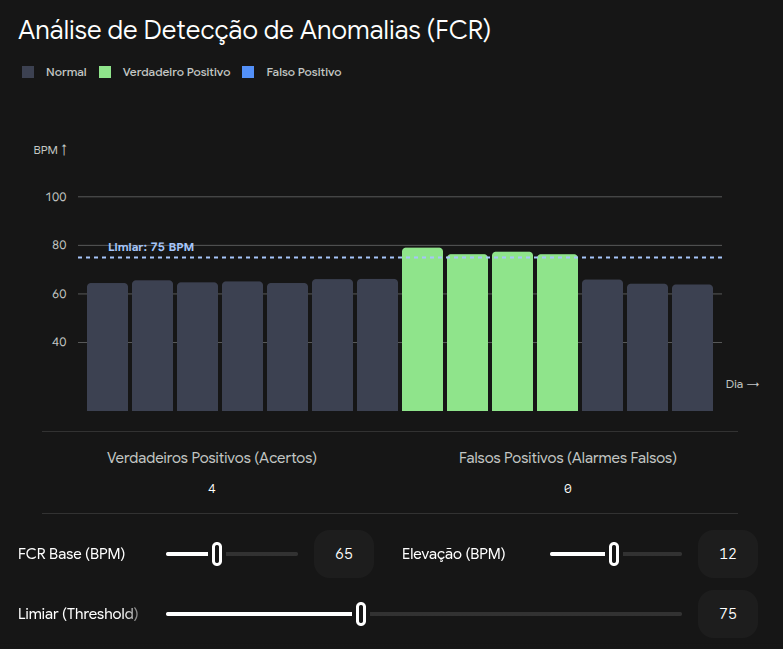
\includegraphics[width=0.8\textwidth]{assets/images/analisedeteccaofcr.png}
        \caption{Simulador de detecção de elevação da FCR para um paciente hipotético. Ajuste FCR Base, Elevação e Limiar (Treshold).}
    \end{figure}
    O projeto tem um escopo excelente. Vocês têm clareza sobre como vão justificar a seleção da técnica de Machine Learning no relatório final da disciplina? Se quiserem, podemos simular agora como estruturar a defesa entre usar KNN vs Árvore de Decisão para esse conjunto de dados!

    \item[Aluno:] Com relação às bases mencionadas, indique o link para cada uma.

    Considerando esse contexto, a equipe em reunião decidiu o seguinte tema, escopo e objetivos:

    TEMA

    Análise Comparativa de Algoritmos Clássicos de Inteligência Artificial na Detecção de Covid-19 através de Padrões de Frequência Cardíaca

    ESCOPO/OBJETIVOS

    A apresentação buscará apresentar alguns algoritmos clássicos da literatura de Inteligência Artificial e confrontá-los para validar uma análise preditiva de diagnóstico positivo de Covid-19 com base na frequência cardíaca em repouso.

    Nesse sentido, tem-se como objetivo a utilização do primeiro algoritmo como o KNN. Dê maior detalhamento em como ele atuaria na resolução da questão.

    \item[Gemini:] Aqui estão os links oficiais para os repositórios abertos que discutimos, fundamentais para a etapa de "Busca de fonte de dados" exigida no trabalho:

    1. Welltory/hrv-covid19: \href{https://github.com/Welltory/hrv-covid19}{repositório no GitHub}
    \textit{Base focada em Variabilidade da Frequência Cardíaca (HRV) e sintomas de usuários de smartwatches durante a pandemia.}
    2. CovIdentify (via Digital Biomarker Discovery Pipeline): \href{https://github.com/DigitalBiomarkerDiscoveryPipeline/CovIdentify}{repositório no GitHub}
    \textit{Projeto liderado pela Duke University focado especificamente em usar dados de dispositivos vestíveis (Fitbit, Apple Watch, Garmin) para prever infecções por Covid-19 usando a Frequência Cardíaca de Repouso (FCR) e contagem de passos.}

    \textbf{O Funcionamento do KNN (K-Nearest Neighbors) no Contexto do Projeto}

    O K-Nearest Neighbors (K-Vizinhos Mais Próximos) é um algoritmo clássico de aprendizado supervisionado baseado na premissa de que "coisas semelhantes estão próximas umas das outras". Ele não constrói um modelo interno complexo (é o que chamamos de \textit{lazy learning} ou aprendizado preguiçoso); ele simplesmente guarda os dados históricos e os usa como mapa de referência no momento da classificação.

    Para o escopo do trabalho de vocês, veja o passo a passo de como ele atuaria na detecção de um padrão de Covid-19:

    \textbf{1. Extração de Características (Features):}
    Não basta passar a data e o BPM bruto para o KNN. Vocês precisariam extrair métricas de cada noite de sono para posicionar esse dia em um "plano cartesiano" (um espaço vetorial multidimensional). Por exemplo:

    \begin{itemize}
        \item Eixo X (Característica 1): Desvio da Frequência Cardíaca de Repouso. (O BPM dessa noite menos a média de BPM do paciente nos últimos 14 dias).
        \item Eixo Y (Característica 2): Tendência de Aceleração. (A diferença do BPM de repouso de hoje em relação ao de ontem).
        \item A contagem de passos (Steps) seria usada na etapa de pré-processamento apenas para garantir que estamos olhando para minutos em que o paciente estava em repouso absoluto.
    \end{itemize}

    \textbf{2. O Mapeamento Histórico:}
    Cada noite de pacientes que já tiveram Covid-19 (dados de treino das bases acima) é plotada nesse espaço. Noites saudáveis tenderão a se agrupar no centro (Desvio 0, Tendência 0). Noites na janela de infecção tenderão a se deslocar para um quadrante de Desvio Positivo e Tendência Positiva.

    \textbf{3. A Chegada de um "Novo Dia":}
    Quando o sistema recebe a leitura do relógio de um paciente em tempo real, ele cria um novo ponto no gráfico com base no desvio daquela noite.

    \textbf{4. Cálculo de Distância e Votação (O Papel do "K"):}
    O algoritmo calcula a distância matemática (como a distância Euclidiana, aquela clássica pitagórica: 
    $\sqrt{(x_2-x_1)^2 + (y_2-y_1)^2}$) entre o "Novo Dia" e todos os dias históricos.
    Em seguida, ele seleciona os K vizinhos mais próximos. Se o seu $K = 5$, ele olha para os 5 dias que tiveram o padrão de batimentos mais parecido com o de hoje. Se 4 desses dias históricos forem rotulados como "Infectados" e apenas 1 como "Saudável", o algoritmo prevê que o paciente está com Covid-19 pela regra da maioria.

    Para que sua equipe possa testar na prática a importância de escolher os eixos (features) e o impacto do parâmetro "K" em zonas fronteiriças (quando um dia tem apenas uma leve alteração cardíaca), construí o simulador abaixo

    \begin{figure}[H]
        \centering
        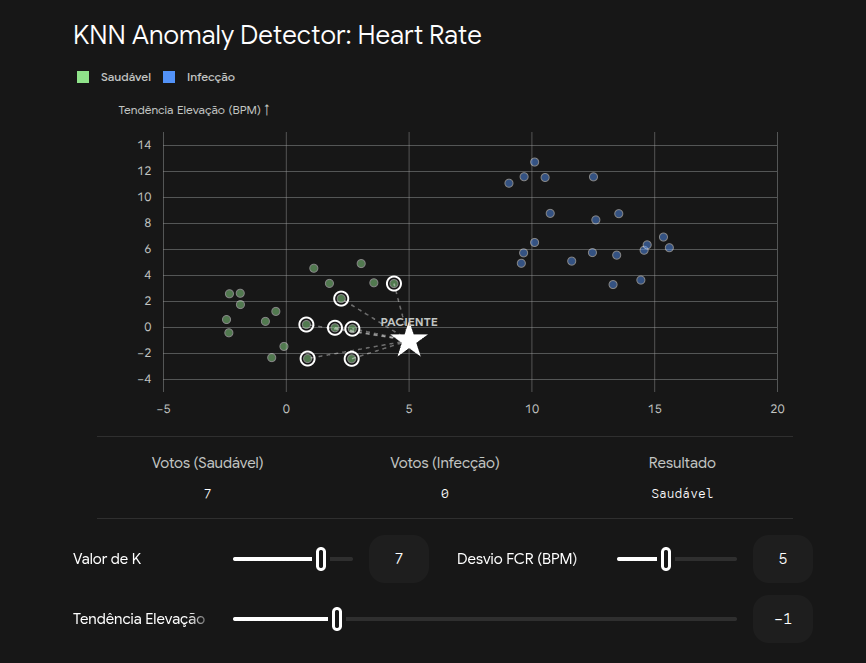
\includegraphics[width=0.8\textwidth]{assets/images/knn.png}
        \caption{Detector de anomalias KNN. Ajuste de Valor de K, Desvio FCR e Tendência de elevação.}
    \end{figure}

    Um ponto de reflexão para o trabalho de vocês: Uma desvantagem do KNN é o custo computacional. Se a base da \textit{Duke University} tem milhões de leituras diárias, calcular a distância geométrica do seu "Novo Dia" para todos esses milhões de pontos pode ser muito lento para um diagnóstico em tempo real no smartwatch. Esse é um excelente ponto de argumentação para a professora sobre os prós e contras que vocês identificarão na "Análise Comparativa" (onde as Árvores de Decisão podem levar vantagem na hora da inferência)!

    \item[Aluno:] Em uma busca, encontramos o seguinte artigo: \href{https://www.nature.com/articles/s41591-021-01593-2}{https://www.nature.com/articles/s41591-021-01593-2}. Como você o avalia para esse projeto? A base de dados utilizada no artigo é alguma das listadas anteriormente ou outra?

    \item[Gemini:] Esse é um achado fantástico! Vocês acabaram de esbarrar em um dos artigos mais importantes e citados mundialmente sobre esse exato tema.

    Para responder de forma direta: a base de dados utilizada nesse artigo não é nenhuma das duas que listamos anteriormente.

    As bases anteriores eram da Duke University (\textit{CovIdentify}) e da \textit{Welltory}. Esse artigo da \textit{Nature Medicine} (liderado pelo laboratório do Dr. Michael Snyder, na Stanford University) utiliza um conjunto de dados próprio, coletado através de um aplicativo criado por eles chamado \textit{MyPHD}. Eles monitoraram mais de 3.300 participantes usando Apple Watch, Fitbit e Garmin.

    Aqui está a minha avaliação de como esse artigo se encaixa no projeto de vocês, pensando na metodologia CRISP-DM:

    \textbf{1. O Padrão Ouro para a "Identificação do Problema"}
    Na primeira etapa do trabalho, vocês precisam justificar o contexto e a validade do problema. Esse artigo prova cientificamente que a premissa de vocês funciona. Eles demonstraram que alertas de alterações na frequência cardíaca em repouso (FCR) ocorreram, em média, 3 dias antes do início dos sintomas em 80\% dos casos de Covid-19 detectados. Citar esse estudo na introdução do trabalho dará um peso acadêmico enorme ao projeto.

    \textbf{2. Inspiração para a Extração de Padrões (Features)}
    O artigo usa exatamente a lógica que discutimos: eles não olham para o batimento bruto, mas sim para o desvio em relação à linha de base do paciente. Eles desenvolveram um algoritmo chamado \textit{NightSignal}, que foca exclusivamente na FCR noturna (filtrando os ruídos de movimento do dia). Isso valida a decisão da sua equipe de usar "dados de repouso - período noturno" associados à contagem de passos nula.

    \textbf{3. Análise Comparativa de Algoritmos}
    O escopo de vocês é realizar uma "Análise Comparativa de Algoritmos Clássicos". O artigo da Stanford menciona o uso de métodos de detecção de anomalias (como o \textit{CuSum} e o \textit{RHRAD}). No relatório do trabalho, vocês podem posicionar o KNN e as Árvores de Decisão (que vocês vão programar) como alternativas a esses algoritmos citados pela \textit{Nature}, comparando a complexidade de implementação e a interpretabilidade de cada abordagem.

    Dica sobre a base de dados: geralmente, os dados brutos de artigos médicos da \textit{Nature} são restritos por questões de privacidade (HIPAA) e exigem solicitações formais ao comitê de ética da universidade para serem acessados. Portanto, para a disciplina, continuem utilizando as bases abertas do GitHub (\textit{CovIdentify} ou \textit{Welltory}), mas usem este artigo da Stanford como o referencial teórico que guia como vocês vão tratar os dados dessas bases abertas.

    \item[Aluno:] Além da KNN, quais são outros algoritmos possíveis de serem implementados para explorar a base de dados e o problema em questão?

    \item[Gemini:] Para enriquecer a \textbf{Análise Comparativa} do seu trabalho e atender perfeitamente à ementa da disciplina de IA, existem outros algoritmos clássicos que se encaixam como uma luva nesse problema de detecção de anomalias cardíacas.

    Como o objetivo é identificar se o padrão de uma determinada noite corresponde a um estado "Saudável" ou de "Infecção (Covid-19)", o problema pode ser abordado tanto via \textbf{Aprendizado Supervisionado} (Classificação) quanto via \textbf{Aprendizado Não Supervisionado} (Agrupamento/Detecção de Anomalias).

    Aqui estão as três melhores opções para a sua equipe confrontar com o KNN:

    \textbf{1. Árvores de Decisão (Decision Trees) --- Supervisionado}
    Em vez de calcular distâncias geométricas como o KNN, a Árvore de Decisão cria regras lógicas de "se-então" a partir dos dados de treino. Ela vai buscar os melhores pontos de corte (limiares) nas suas variáveis para separar os dias saudáveis dos dias de infecção.

    \begin{itemize}
        \item \textbf{Como atuaria no projeto:} O algoritmo analisaria a base de dados e criaria uma estrutura hierárquica. Por exemplo: \textit{Se o Desvio da FCR Noturna for maior que 7 BPM, verifique a Tendência de Elevação. Se a Tendência for maior que 3 BPM, classifique como `Infecção'.}
        \item \textbf{Por que implementar:} É o algoritmo com a maior \textbf{interpretabilidade} de todos. Para a feira do ICMC, vocês podem desenhar a árvore gerada em um banner. O público entenderá instantaneamente a lógica que a IA usou para tomar a decisão, o que resolve um dos grandes desafios de projetos de saúde (explicabilidade).
    \end{itemize}

    \textbf{2. Naive Bayes --- Supervisionado}
    O Naive Bayes é um classificador probabilístico baseado no Teorema de Bayes. Ele assume que todas as características (features) são completamente independentes entre si (daí o termo "Naive" / "Ingênuo").

    \begin{itemize}
        \item \textbf{Como atuaria no projeto:} Ele calcularia a probabilidade prévia de uma pessoa estar infectada na base de dados e a probabilidade de apresentar determinado desvio cardíaco dado que está infectada. Ao receber os dados de uma nova noite, ele calcula a probabilidade \textit{a posteriori}: \textit{``Qual é a probabilidade deste paciente estar com Covid-19 sabendo que a FCR dele subiu 8 BPM hoje?''}
        \item \textbf{Por que implementar:} É extremamente leve computacionalmente e lida muito bem com ruídos isolados. É um excelente contraponto ao KNN, que sofre muito se a base de dados for gigantesca, enquanto o Naive Bayes calcula probabilidades instantaneamente.
    \end{itemize}

    \textbf{3. K-Means --- Não Supervisionado}
    O K-Means é o algoritmo de agrupamento (clustering) mais famoso da literatura. Ao contrário dos anteriores, ele não usa os rótulos (labels) de "Saudável" ou "Covid" durante o treinamento. Ele tenta descobrir padrões ocultos puramente pela geometria dos dados.

    \begin{itemize}
        \item \textbf{Como atuaria no projeto:} Vocês passariam os dados de FCR e tendência de várias noites e pediriam para o algoritmo encontrar $K=2$ grupos (clusters). O K-Means vai definir dois centros geométricos (centroides) e agrupar cada noite ao centroide mais próximo. Ao final, vocês analisam se um dos clusters concentrou naturalmente os dias em que os pacientes estavam doentes.
        \item \textbf{Por que implementar:} Permite demonstrar o poder do aprendizado não supervisionado. Na feira, vocês podem mostrar como a IA consegue separar dias normais de dias anômalos sem que ninguém tenha dito a ela previamente o que era cada coisa.
    \end{itemize}

    \textbf{Entendendo a Fronteira de Decisão: KNN vs. Árvore de Decisão}
    A escolha do algoritmo muda completamente a forma como o "mapa" de diagnóstico é desenhado. Enquanto o KNN cria fronteiras de decisão curvas e complexas (baseadas na proximidade dos vizinhos), a Árvore de Decisão cria cortes estritamente ortogonais (linhas retas horizontais e verticais), pois avalia uma variável por vez.

    Para que a equipe possa visualizar essa diferença matemática crucial antes de codificar, utilizem o simulador interativo abaixo. Ele compara como o KNN e uma estrutura de Árvore de Decisão (por limiares) dividem o espaço de estados de um paciente:
    \begin{figure}[H]
        \centering
        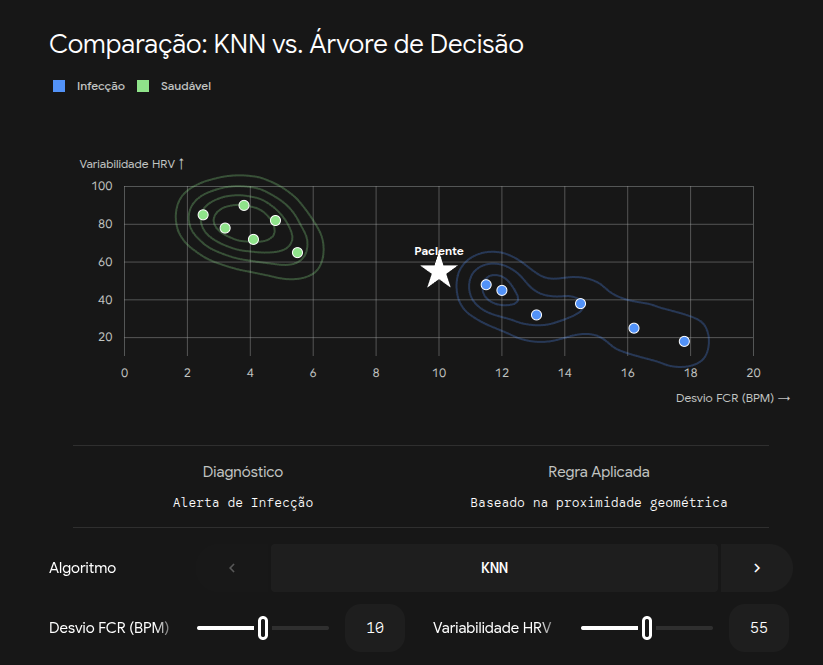
\includegraphics[width=0.8\textwidth]{assets/images/knnvsarvoredecisao.png}
        \caption{Comparação entre KNN e Árvore de Decisão. Ajuste de Desvio FCR e Variabilidade HRV.}
    \end{figure}
    \textbf{Sugestão de Caminho para a Equipe:}
    Para a entrega acadêmica e o relatório da professora, o cenário ideal de \textbf{Análise Comparativa} seria implementar:

    \begin{enumerate}
        \item \textbf{KNN} (representando algoritmos baseados em distância/vizinhança).
        \item \textbf{Árvore de Decisão} (representando algoritmos baseados em regras lógicas e alta interpretabilidade).
    \end{enumerate}

    Isso dará um contraste rico para discutir no artigo do trabalho. Como vocês preferem estruturar o pipeline de pré-processamento para alimentar esses dois modelos?

    \item[Aluno:] Além disso, o projeto propõe a utilização de um terceiro algoritmo. Qual seria outra possibilidade?

    \item[Gemini:] Para fechar a trindade da sua \textbf{Análise Comparativa}, a escolha ideal, que também consta diretamente na ementa da disciplina, é a \textbf{Rede Neural Artificial}, mais especificamente um modelo \textbf{Multi-Layer Perceptron (MLP)}.

    Adicionar uma Rede Neural eleva o nível técnico do projeto da sua equipe no ICMC, criando um espectro perfeito de comparação entre três paradigmas completamente diferentes da IA clássica:

    \begin{enumerate}
        \item \textbf{KNN:} Aprendizado baseado em instâncias (distância geométrica).
        \item \textbf{Árvore de Decisão:} Aprendizado simbólico (regras lógicas claras).
        \item \textbf{Rede Neural (MLP):} Aprendizado conexionista (reconhecimento de padrões não-lineares).
    \end{enumerate}

    Veja como estruturar a defesa da Rede Neural no escopo do trabalho:

    \textbf{Como a Rede Neural atuaria no problema}
    Uma Rede Neural tentará simular matematicamente como o cérebro processa informações. Para os dados dos relógios:

    \begin{itemize}
        \item \textbf{Camada de Entrada (Input Layer):} Recebe as métricas de repouso pré-processadas (ex: desvio da FCR, tendência de elevação, e talvez a média de passos do dia anterior para contexto de fadiga).
        \item \textbf{Camadas Ocultas (Hidden Layers):} Diferente da Árvore de Decisão, que olha uma variável por vez, os "neurônios" ocultos multiplicam e combinam todas as variáveis de entrada simultaneamente, aplicando funções de ativação. Isso permite que a IA identifique padrões altamente complexos e não-lineares, como uma leve taquicardia associada a uma flutuação específica na variabilidade cardíaca que passaria despercebida por regras manuais.
        \item \textbf{Camada de Saída (Output Layer):} Retorna uma probabilidade contínua (ex: 87\% de chance de o paciente estar na janela de infecção da Covid-19).
    \end{itemize}

    \textbf{O Argumento de Arquitetura e Desempenho (O Diferencial do Relatório)}
    Na sua análise comparativa, vocês podem explorar um contraste brutal entre o KNN e as Redes Neurais em relação ao custo computacional de inferência, o que é vital para dispositivos vestíveis (smartwatches).

    O KNN é um modelo "preguiçoso": na hora de prever o resultado de uma nova noite de sono, ele precisa carregar toda a base histórica e calcular distâncias, o que é ineficiente em produção. Já a Rede Neural, uma vez que a etapa custosa de treinamento é concluída, torna a fase de inferência (a previsão no relógio) extremamente leve. A propagação direta (\textit{forward pass}) nada mais é do que uma série de multiplicações de matrizes. Isso permite que o código rodando em Python ou C/C++ seja amplamente otimizado, aproveitando vetorização nativa (instruções SIMD) e paralelização com multithreading para analisar milhares de sinais de pacientes simultaneamente sem gargalos na memória.

    Para visualizar como a Rede Neural desenha limites muito mais fluidos e adaptáveis do que os recortes quadrados de uma Árvore de Decisão, explore o simulador abaixo:

    \begin{figure}[H]
        \centering
        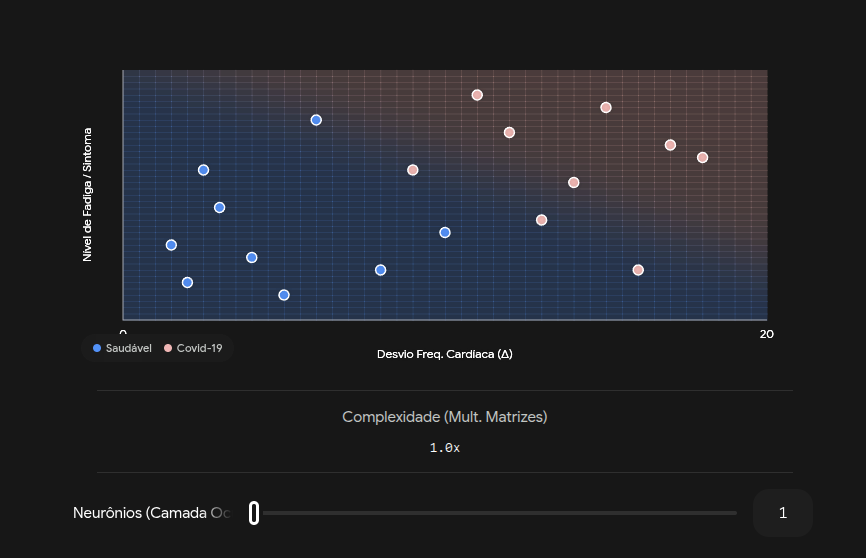
\includegraphics[width=0.8\textwidth]{assets/images/rna.png}
        \caption{Simulador de classificação com Rede Neural. Ajuste de quantidade de neurônios.}
    \end{figure}

    Com esses três algoritmos em mãos (KNN, Árvore de Decisão e MLP), vocês terão o cenário perfeito para aplicar a metodologia CRISP-DM: tratar a base de dados do \textit{Welltory} ou \textit{CovIdentify}, treinar os três modelos com as mesmas \textit{features} da frequência cardíaca noturna e comparar quem obteve os melhores resultados com a maior explicabilidade.

    Considerando as habilidades da equipe e o cronograma do semestre, vocês pretendem utilizar bibliotecas prontas em Python (como o \textit{Scikit-Learn}) para codificar esses três algoritmos, ou a ementa exige a implementação manual da matemática de algum deles a partir do zero?

    \item[Aluno:] Considere toda a discussão e que o tema do projeto será aquele mencionado anteriormente e que a base de dados apresenta, como indicado em algum momento, datas, steps e dados cardíacos de pacientes. Considere também o artigo submetido.

    Elabore um roteiro para a exploração do problema, exploração da base de dados e implementação e desenvolvimento de cada um dos algoritmos (dos 3 discutidos anteriormente), com detalhamento prático de cada um. Nesse roteiro, considere como pipeline de descoberta de conhecimento.

    \item[Gemini:] Este é o momento de amarrar toda a teoria da ementa em um roteiro prático e estruturado. Utilizar o pipeline KDD (Knowledge Discovery in Databases) ou a metodologia CRISP-DM garante que o trabalho não seja apenas um "código que roda", mas uma pesquisa científica rigorosa.

    Abaixo, detalho o roteiro de ponta a ponta, projetado para garantir excelência acadêmica e forte impacto visual na feira de extensões do ICMC, integrando boas práticas de engenharia de software e interação humano-computador na apresentação final.

    \textbf{1. Compreensão do Negócio e do Problema (Business Understanding)}
    Esta é a fundação do relatório. O foco é justificar o porquê da pesquisa.

    Ação Prática: Estruture a introdução do trabalho referenciando o artigo da Nature Medicine (Alavi et al., 2021).
    Definição do Problema: Detectar anomalias fisiológicas antes do aparecimento de sintomas clínicos.
    O Desafio Matemático: Transformar dados brutos de hardware (relógios) em um biomarcador digital (o desvio da Frequência Cardíaca de Repouso - FCR).
    Documentação IA Obrigatória: Registre os prompts exatos usados anteriormente nesta conversa, evidenciando como a IA foi empregada para afunilar o tema de "dados de relógio" para "detecção de anomalias virais via FCR noturna".

    \textbf{2. Compreensão e Exploração dos Dados (Data Understanding)}
    Aqui, o Python brilha. Utilizando bibliotecas como pandas e matplotlib ou seaborn, a equipe deve "conhecer" o formato da base de dados escolhida (como a do CovIdentify).

    Ação Prática: Carregue o dataset e gere estatísticas descritivas.
    Análise Exploratória:
    \begin{itemize}
        \item Verifique a granularidade dos dados (as medições são feitas a cada minuto? A cada hora?).
        \item Plote gráficos de linha mostrando o batimento cardíaco de um paciente ao longo de 24 horas para visualizar a diferença de ruído entre o dia (muitos passos) e a noite.
        \item Identifique dados ausentes (pacientes que tiraram o relógio para carregar).
    \end{itemize}

    \textbf{3. Pré-processamento e Preparação dos Dados (Data Preparation)}
    Esta é a etapa mais crítica. Se os algoritmos receberem "lixo", devolverão "lixo" (garbage in, garbage out).

    Filtro de Repouso Absoluto: Crie uma máscara condicional. Mantenha apenas as linhas onde a coluna Steps é exatamente 0 por uma janela contínua (ex: entre 00h00 e 06h00).
    Agregação: Calcule a mediana dos batimentos dessa janela noturna para gerar a variável FCR\_Diaria.
    Criação de Features (Engenharia de Atributos):
    \begin{itemize}
        \item \textbf{Linha de Base:} Calcule a média móvel da FCR\_Diaria dos últimos 14 ou 21 dias do paciente.
        \item \textbf{Desvio (Feature 1):} Subtraia a linha de base da FCR\_Diaria atual. (Quanto o coração acelerou em relação ao "normal" dessa pessoa?).
        \item \textbf{Tendência (Feature 2):} Subtraia a FCR\_Diaria de hoje da de ontem. (A aceleração está subindo?).
    \end{itemize}
    Rotulação (Labeling): Usando a data do teste de Covid-19, marque os dias de $D-3$ até $D+4$ do teste como 1 (Infecção) e o restante como 0 (Saudável).
    Normalização: Aplique um StandardScaler (Z-score) para garantir que todas as variáveis estejam na mesma escala, passo fundamental antes de rodar algoritmos baseados em distância.

    \textbf{4. Modelagem: Implementação dos Algoritmos (Modeling)}
    Divida o dataset em dados de treino (ex: 70\%) e teste (30\%). A implementação pode ser feita com o scikit-learn em Python.

    \textbf{A. K-Nearest Neighbors (KNN)}
    Implementação: KNeighborsClassifier.
    Ajuste de Hiperpa-\\râmetros: Teste diferentes valores de $K$ (3, 5, 7, 9) e diferentes métricas de distância (Euclidiana vs. Manhattan).
    Detalhamento Prático: Avalie o tempo que o KNN leva para prever um novo dado. Demonstre no relatório como o custo computacional ($\mathcal{O}(N \times D)$) escala com o aumento do banco de dados, o que seria um gargalo para uso nativo no hardware do smartwatch.

    \textbf{B. Árvores de Decisão (Decision Trees)}
    Implementação: DecisionTreeClassifier.
    Ajuste de Hiperparâmetros: Controle a profundidade máxima (max\_depth) para evitar sobreajuste (overfitting), garantindo que a árvore não crie regras específicas demais para os dados de treino.
    Detalhamento Prático: Exporte a árvore gerada usando a função plot\_tree. O grande trunfo aqui é a transparência: o algoritmo entregará exatamente o limiar em BPM que separa um dia saudável de um dia doente.

    \textbf{C. Rede Neural Artificial (Multi-Layer Perceptron - MLP)}
    Implementação: MLPClassifier.
    Arquitetura: Inicie com uma configuração enxuta (ex: uma camada oculta com 8 a 16 neurônios e função de ativação ReLU).
    Detalhamento Prático: Treine o modelo monitorando a curva de perda (loss curve). No relatório, contraste a complexidade matemática da MLP — que cria fronteiras de decisão não-lineares — com a simplicidade da Árvore. Ressalte que, após o treino, a inferência (uma série de multiplicações de matrizes) é extremamente rápida e pode ser facilmente otimizada em linguagens de baixo nível como C ou C++ diretamente no firmware de um dispositivo embarcado.

    \textbf{5. Avaliação Comparativa (Evaluation)}
    Não basta olhar apenas para a "Acurácia". Em problemas de detecção de doenças, o conjunto de dados é desbalanceado (há muito mais dias saudáveis do que dias doentes).
    Métricas Necessárias:
    \begin{itemize}
        \item \textbf{Sensibilidade (Recall):} Dos dias que a pessoa realmente estava com Covid-19, quantos o modelo detectou? (Evitar Falsos Negativos).
        \item \textbf{Precisão (Precision):} Quando o modelo dispara o alarme de Covid-19, qual a chance de ser real e não apenas uma noite de estresse comum? (Evitar Falsos Positivos).
        \item \textbf{F1-Score:} A média harmônica entre os dois.
        \item \textbf{Matriz de Confusão:} Gere e plote as matrizes de confusão para os três algoritmos. Isso será visualmente excelente para colocar nos slides ou banners.
    \end{itemize}

    \textbf{6. Implantação e Apresentação (Deployment / HCI)}
    Para o ICMC, o projeto ganha vida se o público puder interagir com os resultados.
    Ação Prática: Em vez de mostrar apenas linhas de código e métricas brutas, crie um pequeno dashboard visual (usando Streamlit ou Dash no Python).
    Interatividade: Permita que o usuário da feira mova um slider simulando o seu próprio batimento cardíaco noturno e veja, em tempo real, como os três algoritmos divergem ou concordam no diagnóstico. Isso materializa o impacto da Inteligência Artificial em soluções de saúde e valida a excelência do trabalho perante os avaliadores.

    Com esse roteiro estruturado, por onde a equipe prefere iniciar a execução: gostariam de discutir o código base em Python para fazer o filtro de repouso na base de dados, ou preferem debater como baixar e formatar os dados do CovIdentify ou Welltory?

    \item[Aluno:] Agora quanto aos dados, considerando que temos dados de 20 pacientes ao longo de um período, como dividir em quantidade dados que servirão para validação e quantos servirão para treinamento?

    \item[Gemini:] Uma base com 20 pacientes é excelente para uma prova de conceito, mas exige um cuidado cirúrgico na hora da divisão. Em problemas de saúde e séries temporais, a forma como você corta os dados define se o seu modelo está realmente aprendendo ou apenas ``decorando'' os pacientes.

    \textbf{A Armadilha do Vazamento de Dados (Data Leakage)}

    O erro mais comum ao iniciar um projeto de aprendizado de máquina é pegar todas as linhas da base de dados (por exemplo, 600 dias no total) e embaralhar tudo, mandando 70\% das linhas para treino e 30\% para teste.

    Se o ``Paciente 1'' tiver dias tanto no conjunto de treinamento quanto no conjunto de validação, os algoritmos (especialmente o KNN e a Rede Neural) não vão aprender a generalizar o padrão fisiológico da Covid-19. Eles vão simplesmente memorizar a frequência cardíaca basal específica do Paciente 1. Na hora da validação, a métrica de acurácia será artificialmente alta, mas o modelo falhará no mundo real quando um usuário inédito colocar o relógio.

    \textbf{Abordagem 1: Divisão por Sujeito (Subject-wise Split)}

    A regra de ouro neste cenário é: \textbf{a divisão deve ser feita na contagem de indivíduos, mantendo o histórico de cada paciente intacto e inseparável}. Para 20 pacientes, as proporções clássicas aplicadas na indústria ficam assim:

    \begin{center}
    \begin{tabular}{|c|c|c|p{7cm}|}
        \hline
        \textbf{Proporção} & \textbf{Treinamento} & \textbf{Validação / Teste} & \textbf{Contexto Ideal} \\
        \hline
        70/30 & 14 pacientes & 6 pacientes & Ideal se cada indivíduo possuir muitos meses ininterruptos de dados gravados. \\
        \hline
        80/20 & 16 pacientes & 4 pacientes & Recomendado para maximizar a extração de padrões em bases numéricas menores. \\
        \hline
    \end{tabular}
    \end{center}

    \textbf{Abordagem 2: Validação Cruzada (Leave-One-Subject-Out)}

    Como 20 pacientes é uma amostragem relativamente pequena para treinar modelos mais complexos como a MLP, cada paciente deixado de fora do treino faz muita falta na construção das sinapses da rede. A técnica mais rigorosa e robusta para contornar isso, que agregaria um peso científico enorme ao relatório final, é o \textbf{Leave-One-Subject-Out (LOSO)}.

    Nesta técnica, em vez de fazer um único corte estático, o pipeline realiza o treinamento 20 vezes sequenciais:

    \begin{itemize}
        \item Na rodada 1, o modelo treina com os dados de 19 pacientes e tenta prever os dias de infecção exclusivamente do Paciente 1.
        \item Na rodada 2, o modelo treina com 19 pacientes (agora incluindo o Paciente 1) e tenta prever o Paciente 2.
        \item O ciclo se repete até o Paciente 20.
    \end{itemize}

    No final, você calcula a média de acerto de todas as 20 rodadas. Isso garante que o modelo usou 100\% da base de dados para validação, sempre simulando o cenário real de ``um novo relógio pareado por um usuário completamente desconhecido''. Bibliotecas em Python como o Scikit-Learn possuem o módulo \textit{LeaveOneGroupOut} para implementar essa lógica rapidamente.

    Considerando que uma base de monitoramento contínuo gera muitos dias com o rótulo ``saudável'' e apenas uma pequena janela de dias com ``infecção'', como a equipe pretende lidar com o desbalanceamento absoluto dessas classes na hora de passar esses dados para o treinamento?
\end{description}